% To compile, run PDFLaTeX, then bibtex, then PDFLaTex again


\documentclass[conference]{IEEEtran}
\IEEEoverridecommandlockouts
\usepackage{cite}
\usepackage{amsmath,amssymb,amsfonts}
\usepackage{algorithmic}
\usepackage{graphicx}
\usepackage{textcomp}
\usepackage{xcolor}
\usepackage{float}
\usepackage{hyperref} % Adding hyperref for references
\usepackage{url}

\newcommand{\BibTeX}{\textrm{B \kern -.05em \textsc{i \kern -.025em b} \kern -.08em
T \kern -.1667em \lower .7ex \hbox{E} \kern -.125emX}}
\begin{document}


    \title{Open-Source Radiation Hardening Simulator: Design, Implementation, and Applications}

    \author{
        \IEEEauthorblockN{
        Collin Lambert,
        Jacob Anderson,
        David Nichols,
        Parker Allred,
        Shiuh-hua Wood Chiang, \textit{Senior Member, IEEE},
        }
        \IEEEauthorblockN{
        Jeffrey Goeders, \textit{Senior Member, IEEE},
        and Mike Wirthlin, \textit{Senior Member, IEEE}
        }
    }

    \maketitle

    \begin{abstract}
        This paper presents the design, implementation, and applications of an open-source radiation hardening simulator developed using XSchem and Ngspice.
        The simulator aims to address the challenges of simulating radiation effects on electronic circuits by providing a comprehensive library and user-friendly interface.
        The project integrates core modules for radiation effect simulation, including Single Event Effects (SEE), along with thorough documentation and examples to support users in their research and development efforts.
        Preliminary tests demonstrate the simulator's accuracy in modeling radiation effects, offering significant potential for future research and development.
    \end{abstract}

    \begin{IEEEkeywords}
        radiation hardening, electronic circuits, fault injection, simulation, XSchem, NGSpice, PN-junction, reverse bias, photocurrent
    \end{IEEEkeywords}


    \section{Introduction}\label{sec:introduction}
    Radiation can induce a variety of faults and errors in electronic components, leading to system failures.
    To prevent such system failures, accurate simulations of radiation effects on electronic circuits are of utmost import. These simulations are a key part in the development of robust systems in space, nuclear, and other radiation-prone environments.
    Thus, understanding and mitigating these effects is essential for ensuring the reliability of electronic systems~\cite{Wrobel2011, Florian1986}.

    Natural radiation is known to be a source of microelectronics failure, impacting various applications from aerospace to ground-level electronics.
    To predict the reliability of these devices, tools like MC-ORACLE and RADSPICE have been developed to simulate the effects of radiation on microelectronic materials~\cite{Wrobel2011, Florian1986}.

    In this paper, we introduce an open-source radiation hardening simulator that leverages XSchem and NGSpice.
    This tool is designed to simulate and analyze the effects of radiation on electronic circuits, and aims to facilitate the development and testing of radiation-hardened designs.
    Our approach includes simulating Single Event Effects (SEE) using advanced models such as adaptive double exponential current sources to improve the accuracy of simulations~\cite{Pepper1990}.

    The paper is structured as follows: Section II provides an overview of the project, including its background, objectives, and scope.
    Section III details the methodology and implementation, describing the integration of XSchem, NGSpice, and custom-developed modules.
    Section IV presents the testing, results, and discussion.
    Finally, Section V concludes the paper and outlines future work.


    \section{Project Overview}\label{sec:project-overview}
    This section provides an overview of the project, including structure, background, objectives, and scope.

    \subsection{Background}\label{subsec:background}
    
   	Single-Event Effects (SEEs) are some of the most commonly simulated radiation effects. One single-event effect of interest are transients resulting from photocurrent generation. When a radiation particle passes through silicon, it generates electron hole pairs along the length of the radiation track. In most cases, there is no strong electric field to separate these charges and the electron hole pairs recombine randomly. If, however, the electron hole pairs are generated in the proximity of a strong electric field, such as a reverse biased PN junction, the electrons and holes can be separated before recombination can occur. These charges are swept out of the junction which creates a photocurrent in the circuit. This photocurrent then generates voltage transients in the circuit. These transients are one of many single-event effects. Fig.~\ref{fig:cmos_inverter} depicts a radiation event taking place in a CMOS inverter.
    
    \begin{figure}[htbp]
        \centering
        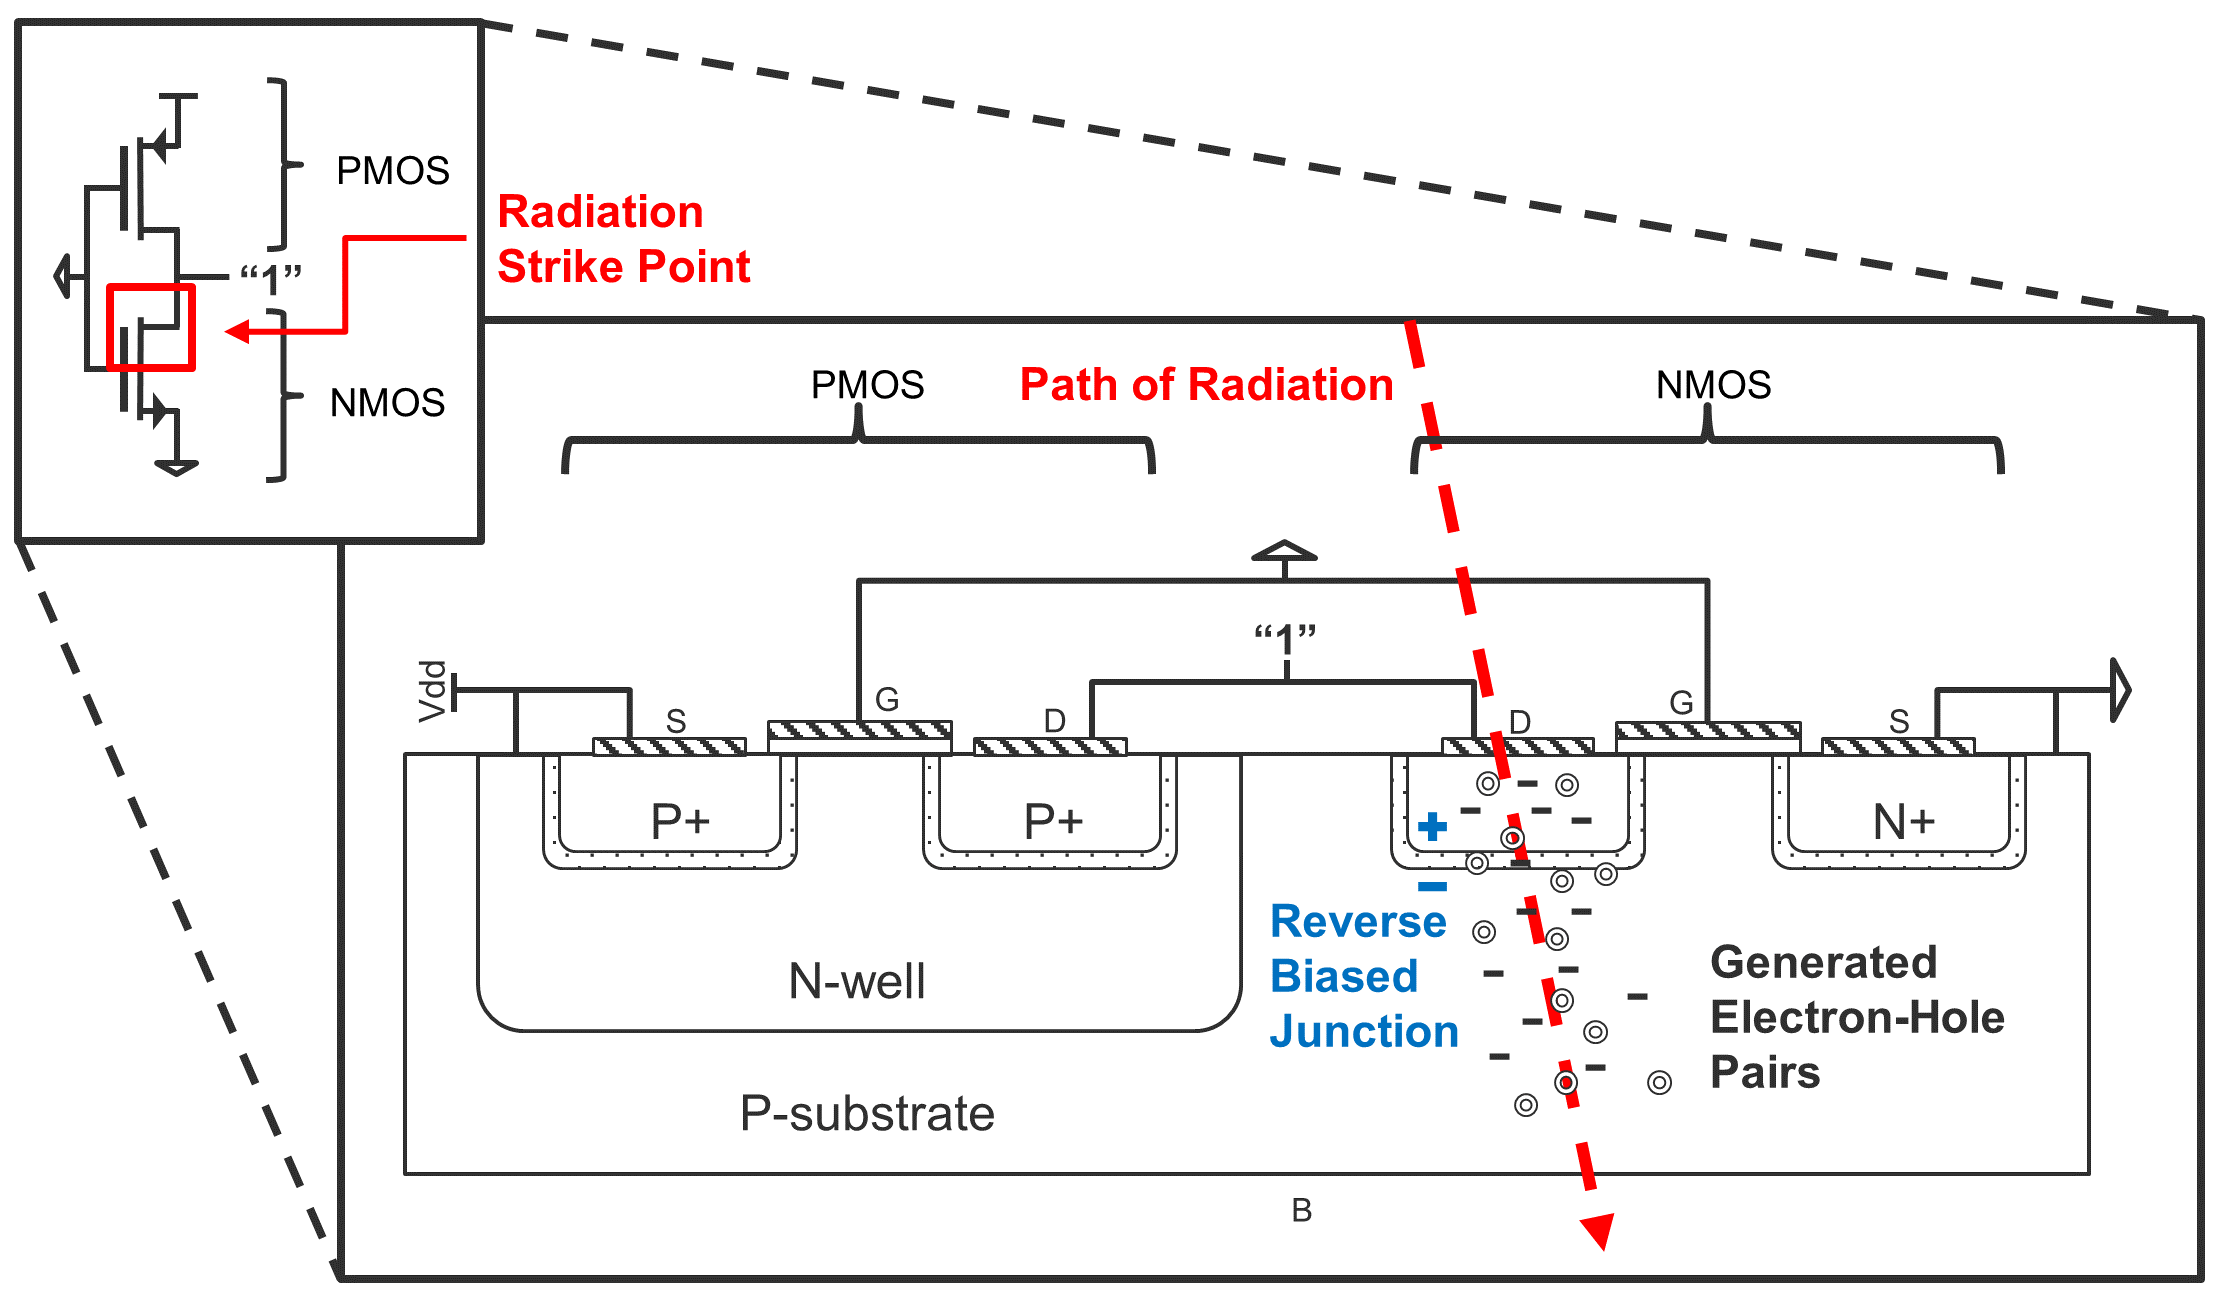
\includegraphics[width=1\linewidth]{Inverter_Image_B_W_cropped}
        \caption{Radiation event in a CMOS Inverter. In the above configuration, the drain of the NMOS transistor is held in a reverse bias condition. When radiation stikes the aforementioned drain region, electron-hole pairs are generated along the radiation track. A photocurrent is then generated due to the reverse bias condition, thus creating voltage transients.}
        \label{fig:cmos_inverter}
    \end{figure}
    
        \subsection{Project Scope and Objectives}\label{subsec:project-scope-and-objectives}
    There are multiple existing Radiation-Hardened SPICE simulators; however, these simulators are not open-sourced, limiting their accessibility.
    The primary objective of this project is to develop an open-source, radiation-effects SPICE simulator that is both user-friendly and accurate in its modeling capabilities.
    
    \subsection{Structure}\label{subsec:project-structure}
    
        \begin{figure}[htbp]
        \centering
        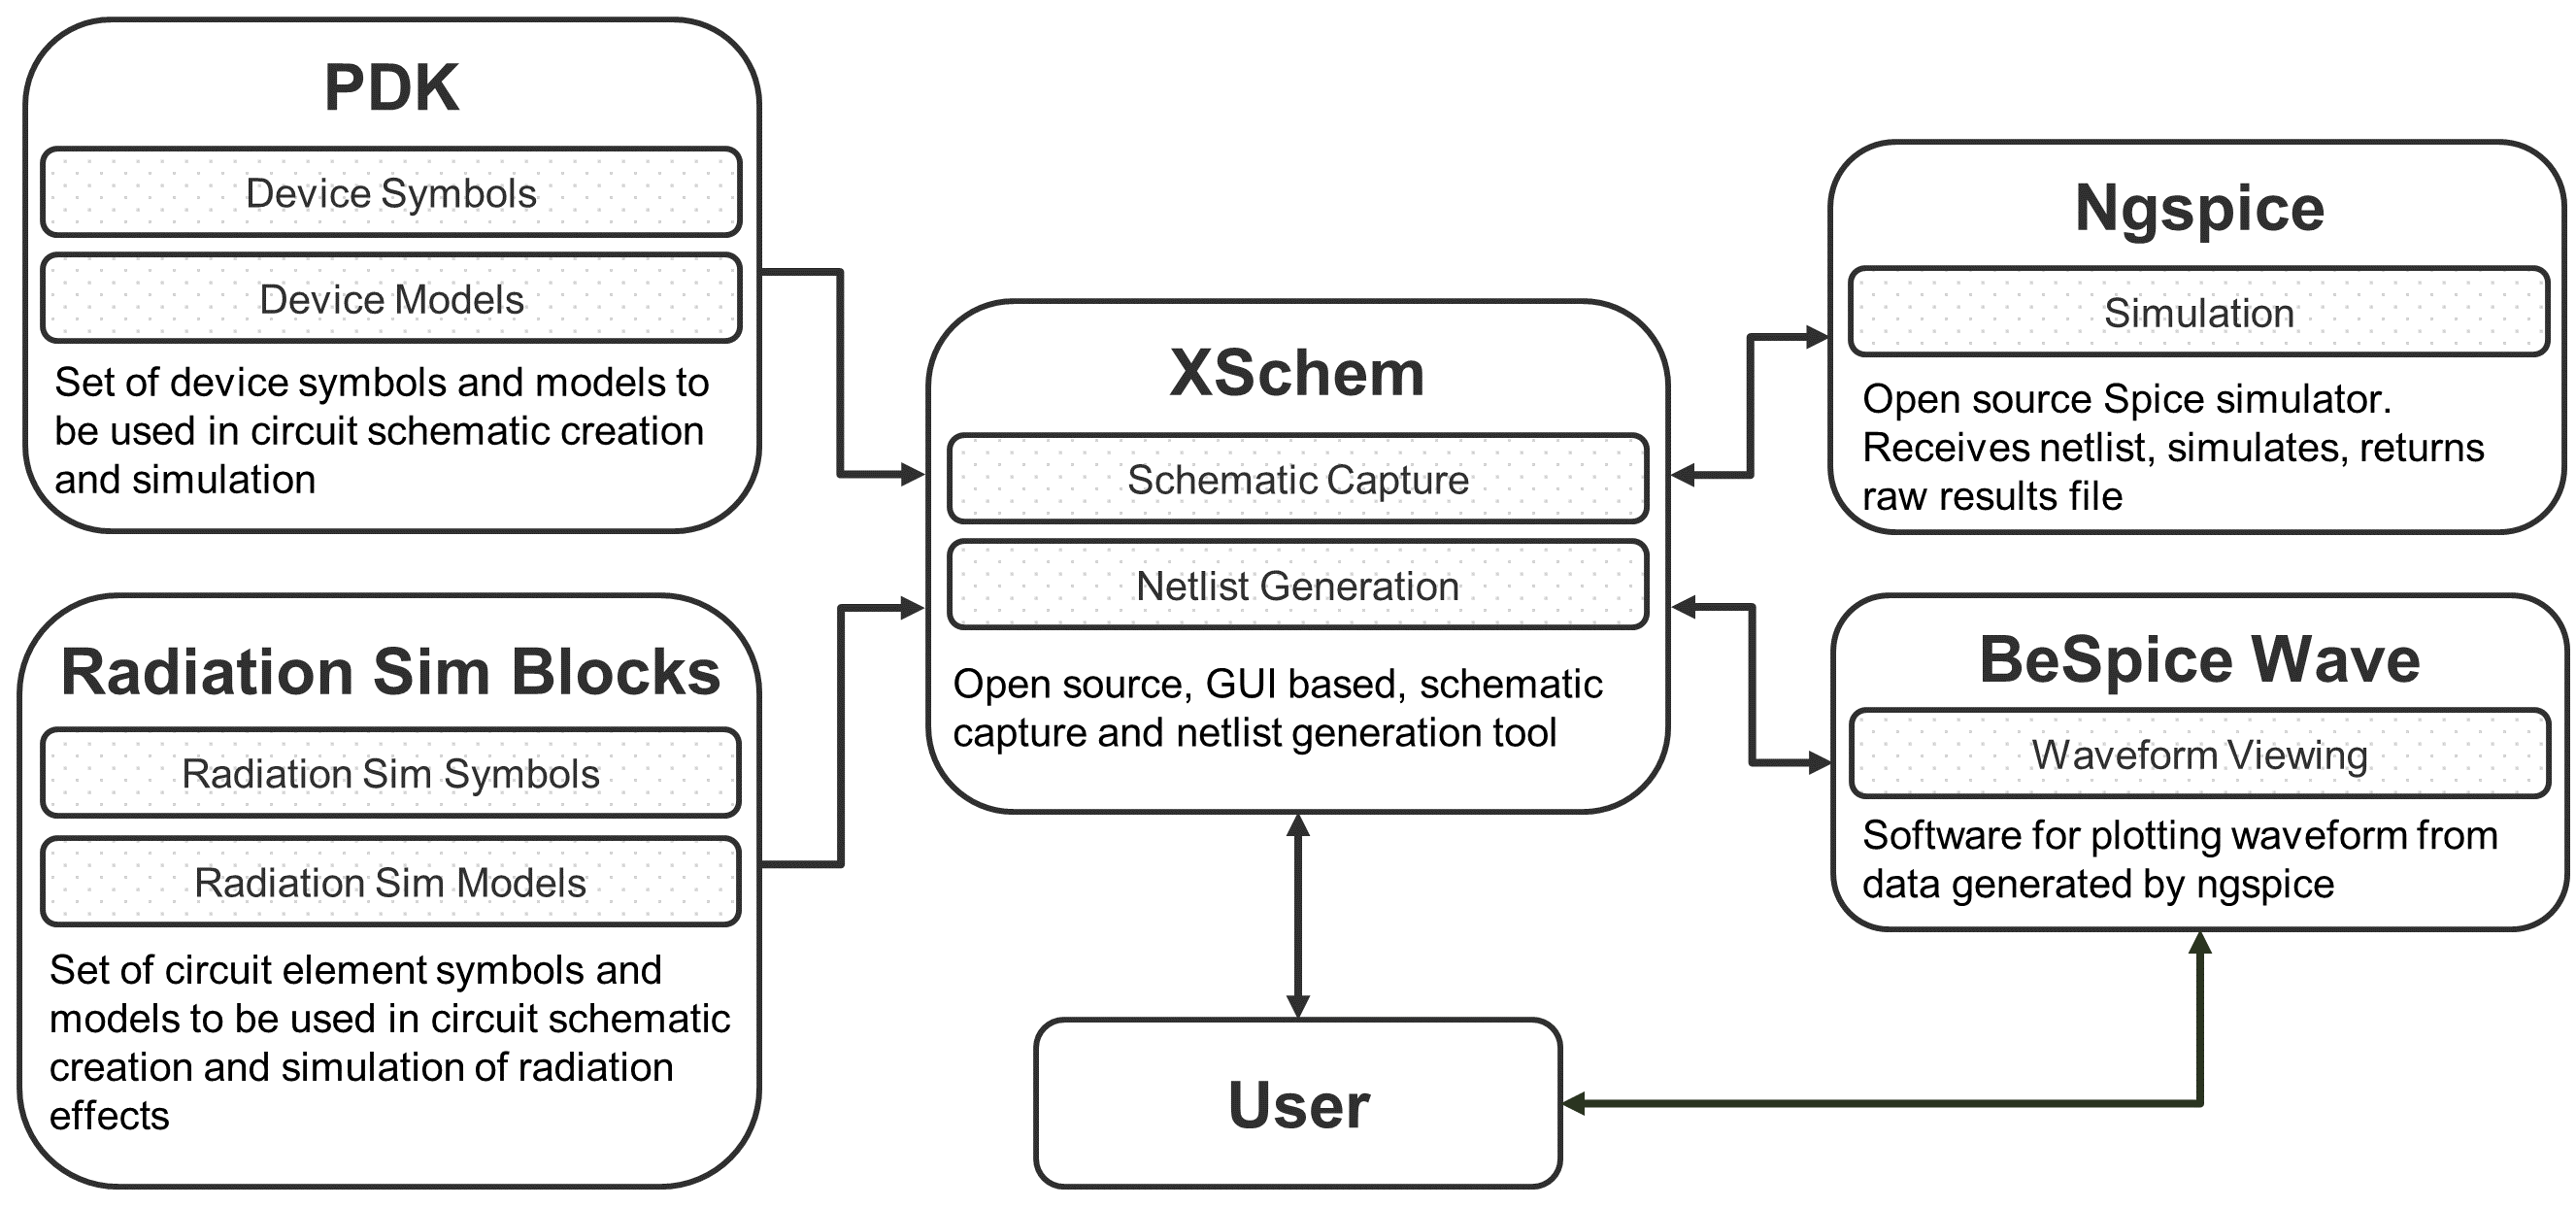
\includegraphics[width=0.95\linewidth]{Block_Diagram_B_W_cropped}
        \caption{Interaction Diagram. This figure shows how different components of the project interact with each other.}
        \label{fig:interaction_diagram}
    \end{figure}
    
    To facilitate easy schematic creation and simulation, we've chosen to use an open source program called Xschem. Xschem provides a GUI interface for drawing circuits, generating netlists, running simulations, and viewing waveforms. We've created a set of radiation simulation blocks that can be imported into Xschem as components. These components can then be included in schematics and simulated. Once a schematic is created, Xschem generates a netlist, sends the netlist to ngspice to simulate, receives the results from ngspice, and finally sends the results to an external waveform viewer (in this case we are using BeSpice Wave). The interactions between each component of this project are detailed in Fig. \ref{fig:interaction_diagram}.
    
	\begin{figure}[htbp]
        \centering
        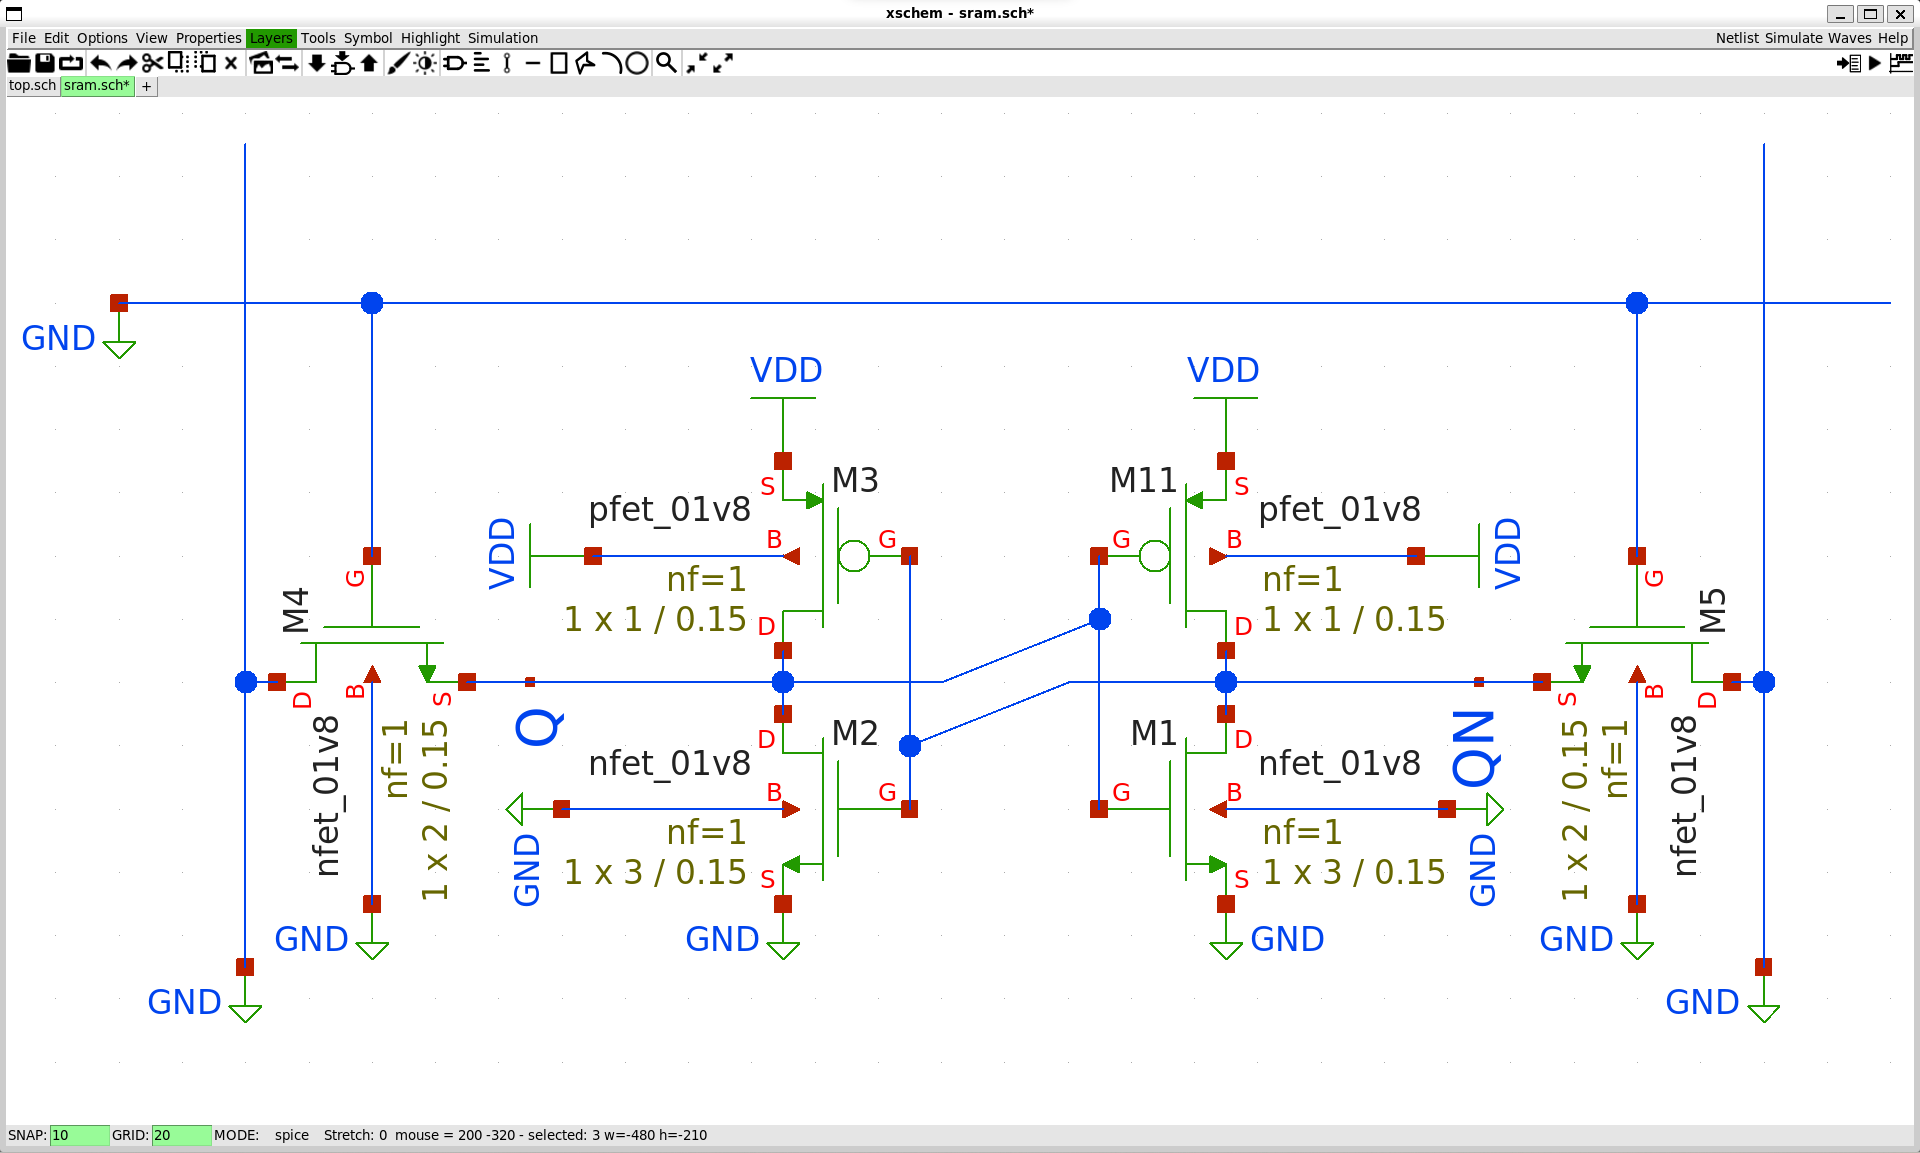
\includegraphics[width=0.95\linewidth]{xschem_env}
        \caption{Xschem schematic capture environment}
        \label{fig:xschem}
    \end{figure}
    
    \begin{figure}[htbp]
        \centering
        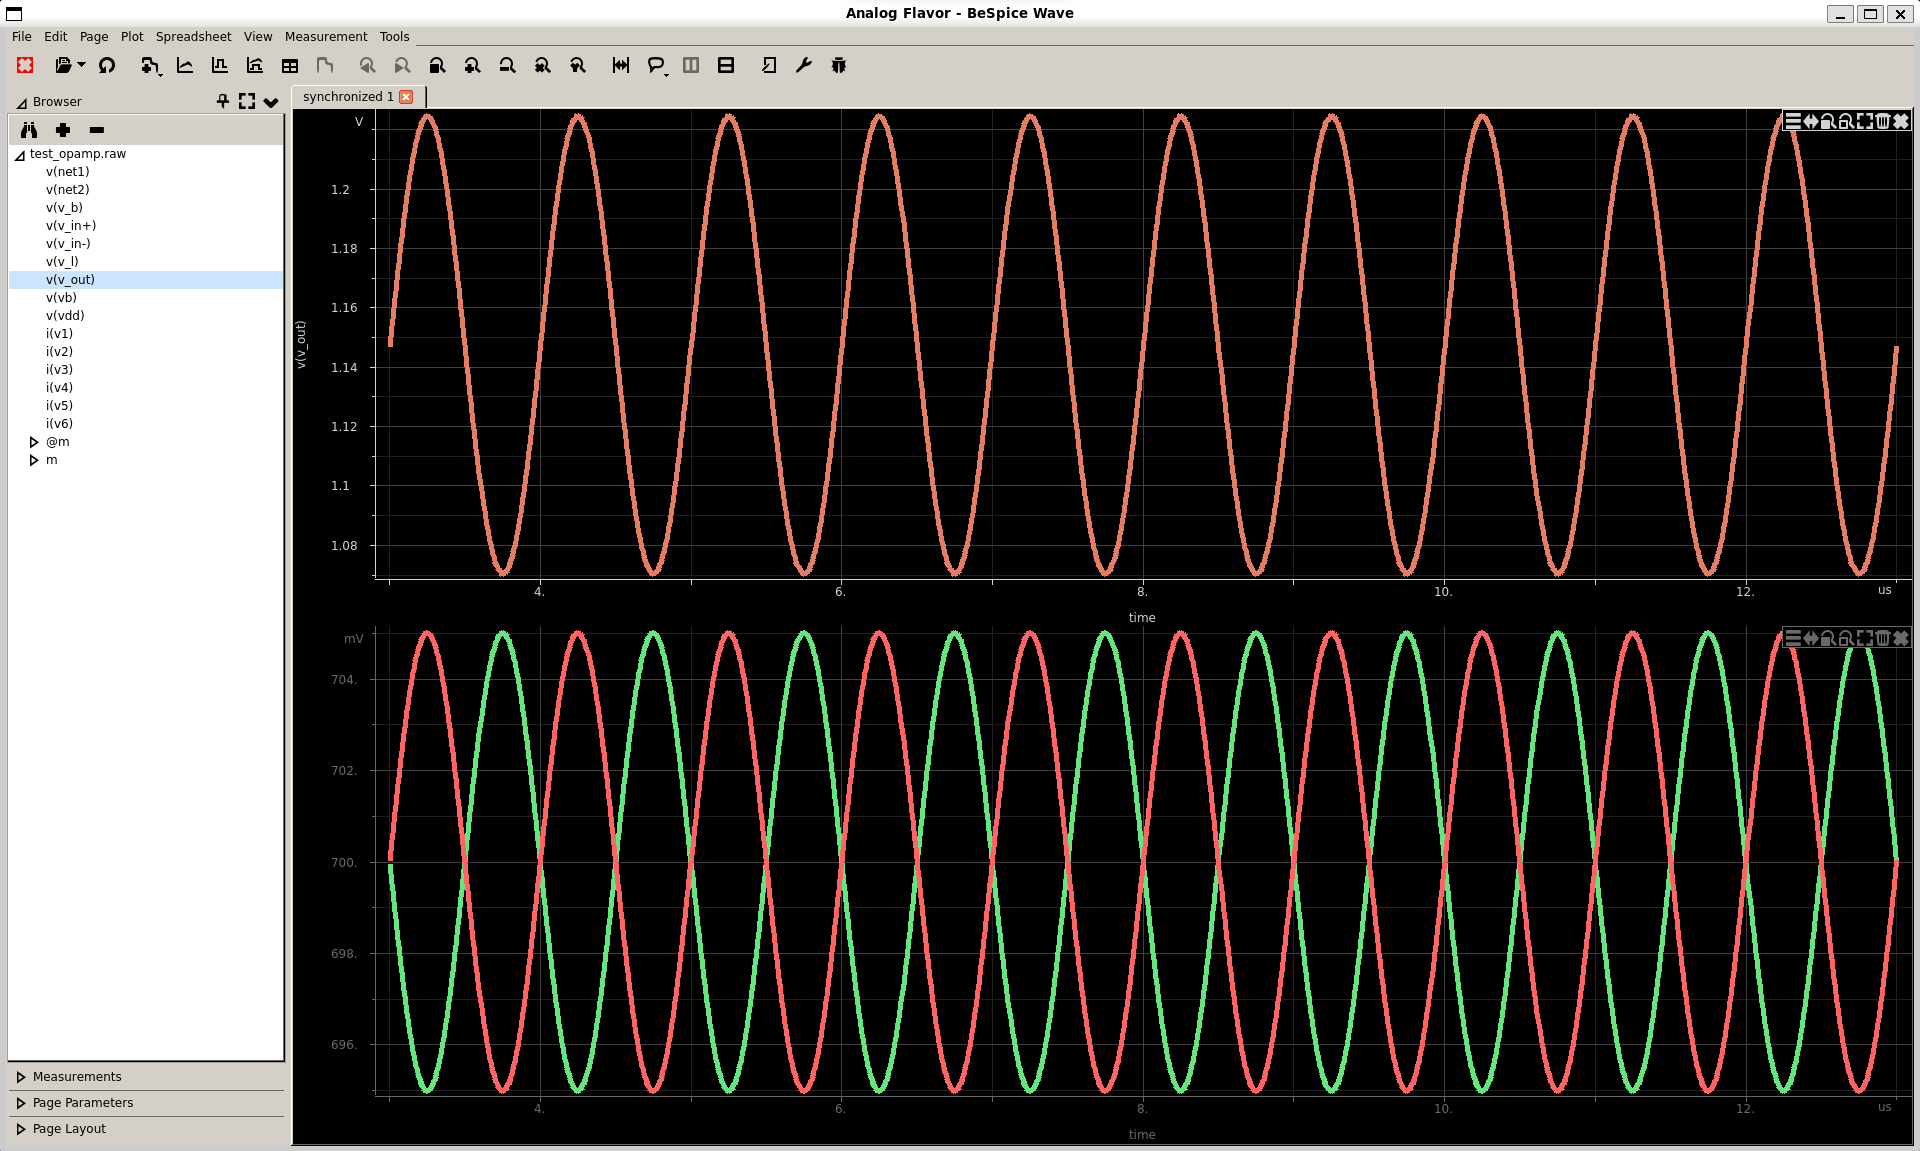
\includegraphics[width=0.95\linewidth]{bespicewave}
        \caption{BeSpice Wave external waveform viewer. Can be opened directly from withing Xschem}
        \label{fig:bespicewave}
    \end{figure}


    \section{Methodology and Implementation}\label{sec:methodology-and-implementation}
    Our simulator presents a user-friendly and intuitive experience to the user.
    To effectuate this, we implement each radiation effect as a block that can be placed and connected to other components in XSchem.
    A description of each block is as follows:

    

    \subsection{Single Event Effect [SEE] Simulation}\label{subsec:single-event-effect-[see]-simulation}

    \subsubsection{Double Exponential Current Source}
    A simple way to model the photo-current generated in a reverse biased pn junction due to a radiation strike is with a double exponential current source.
    This method has existed for decades and is widely used.
    Fig.~\ref{fig:double_exp} depicts a double exponential waveform.

    \begin{figure}[htbp]
        \centering
        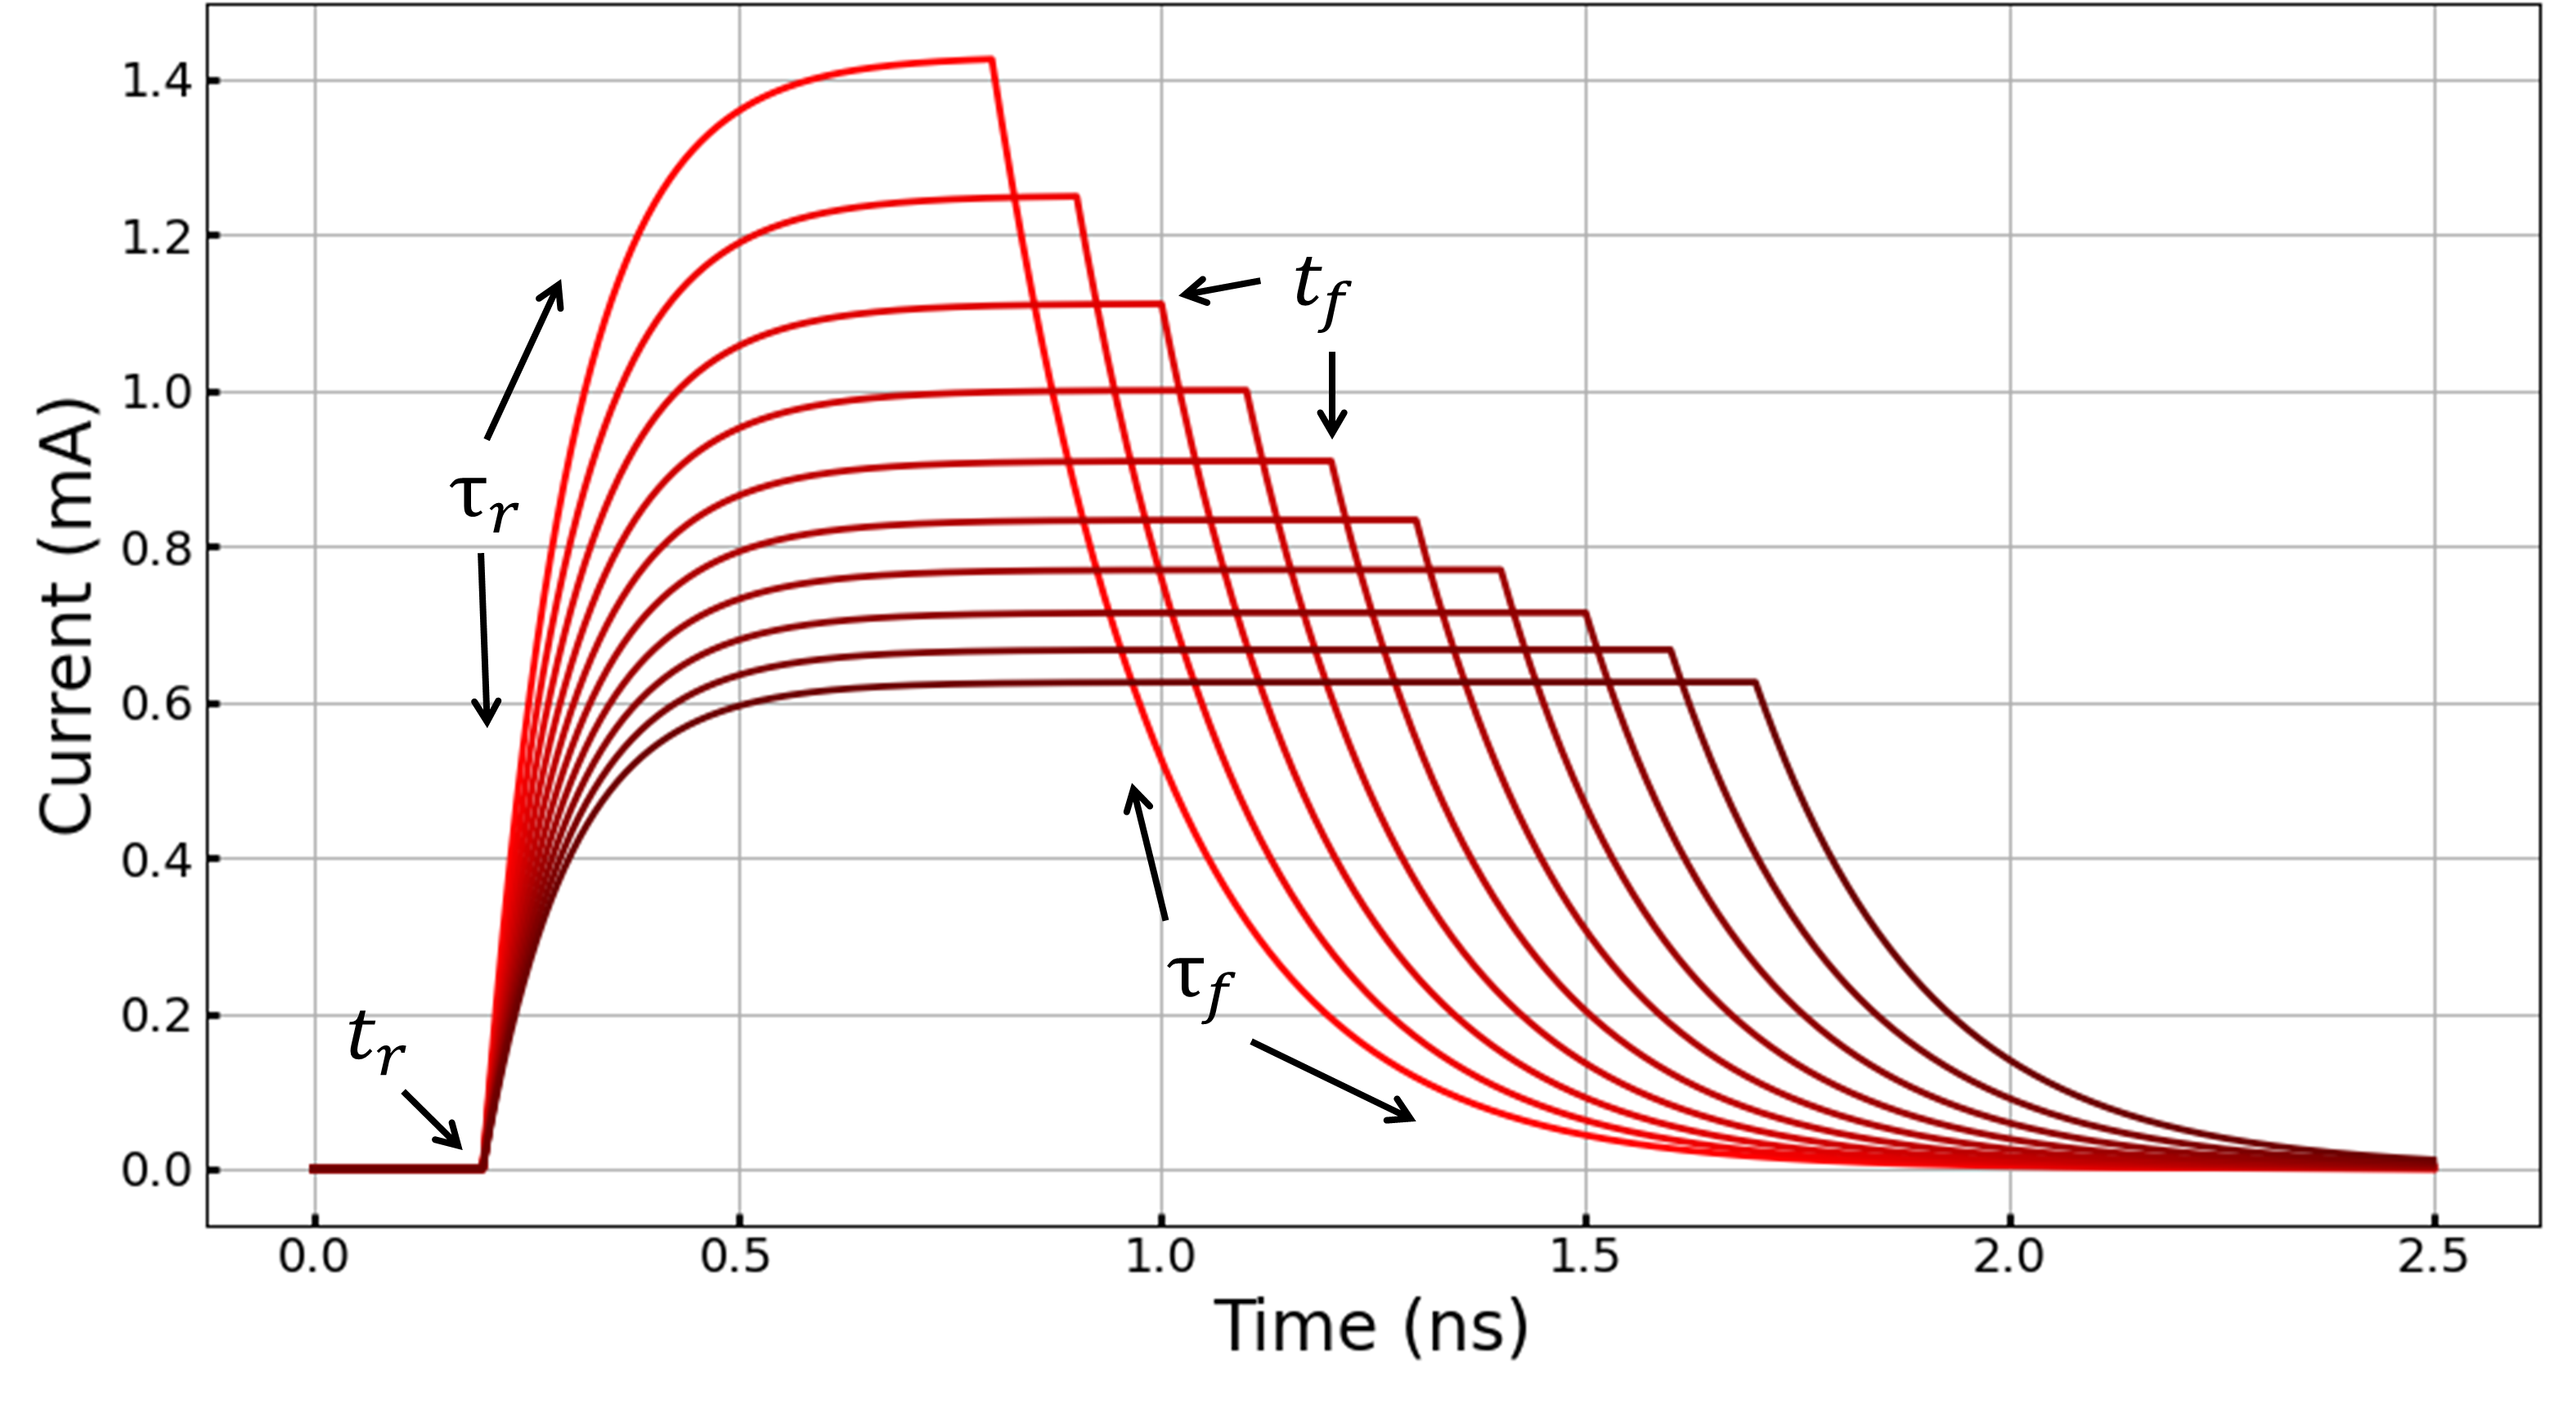
\includegraphics[width=0.95\linewidth]{double_exp_param_no_title}
        \caption{Family of double exponential curves. The area under the curve represents total charge delivered. Each curve in this plot has the same area underneath it (total charge). This demonstrates the ability of the double exponential radiation simulation block to be customized by adjusting various parameters such as \(t_r\), \(t_f\), \(\tau_r\), and \(\tau_f\).}
        \label{fig:double_exp}
    \end{figure}
    
    The equations that govern the behavior of such a double exponential current source are given in equations (\ref{eq:Ipeak}) and (\ref{eq:ISRC})
    
    \begin{equation}
        I_{\text{peak}} = \frac{Q_{\text{tot}}}{[(t_f - t_r) - \tau_r + \tau_f]}\label{eq:Ipeak}
    \end{equation}

    \begin{equation}
        I = \begin{cases}
                      0, & t < t_r \\
                      I_{\text{peak}}\left(1 - e^{\frac{-(t - t_r)}{\tau_r}}\right), & t_r \leq t < t_f \\
                      I_{\text{peak}}\left(e^{\frac{-(t - t_f)}{\tau_f}} - e^{\frac{-(t - t_r)}{\tau_r}}\right), & t_f > t
        \end{cases}\label{eq:ISRC}
    \end{equation}
    
	\vspace{1em}
    
    \begin{itemize}
        \item[] \(t_r\) - Simulation time at which charge injection begins

        \item[] \(t_f\) - Simulation time at which charge injection halts

        \item[] \(\tau_r\) - Rise time constant of \(I_{SRC}\)

        \item[] \(\tau_f\) - Fall time constant of \(I_{SRC}\)

        \item[] \(Q_{tot}\) - Total charge to be injected into the node
    \end{itemize}
    
    \vspace{1em}

    \subsubsection{Dual Double Exponential Current Source}
    A limitation of the simple double exponential current source is that it can be inaccurate in some scenarios.
    It has been found that a more realistic photo-current waveform consists of an initial peak followed by a plateau region caused by limitations of PMOS drive current in CMOS circuitry, and a final drop off.
    This waveform can be represented by adding two double exponential current sources together resulting in a dual double exponential current source.~\cite{Black2015}.
    Fig.~\ref{fig:dual_double_exp} depicts a dual double exponential waveform

    \begin{figure}[htbp]
        \centering
        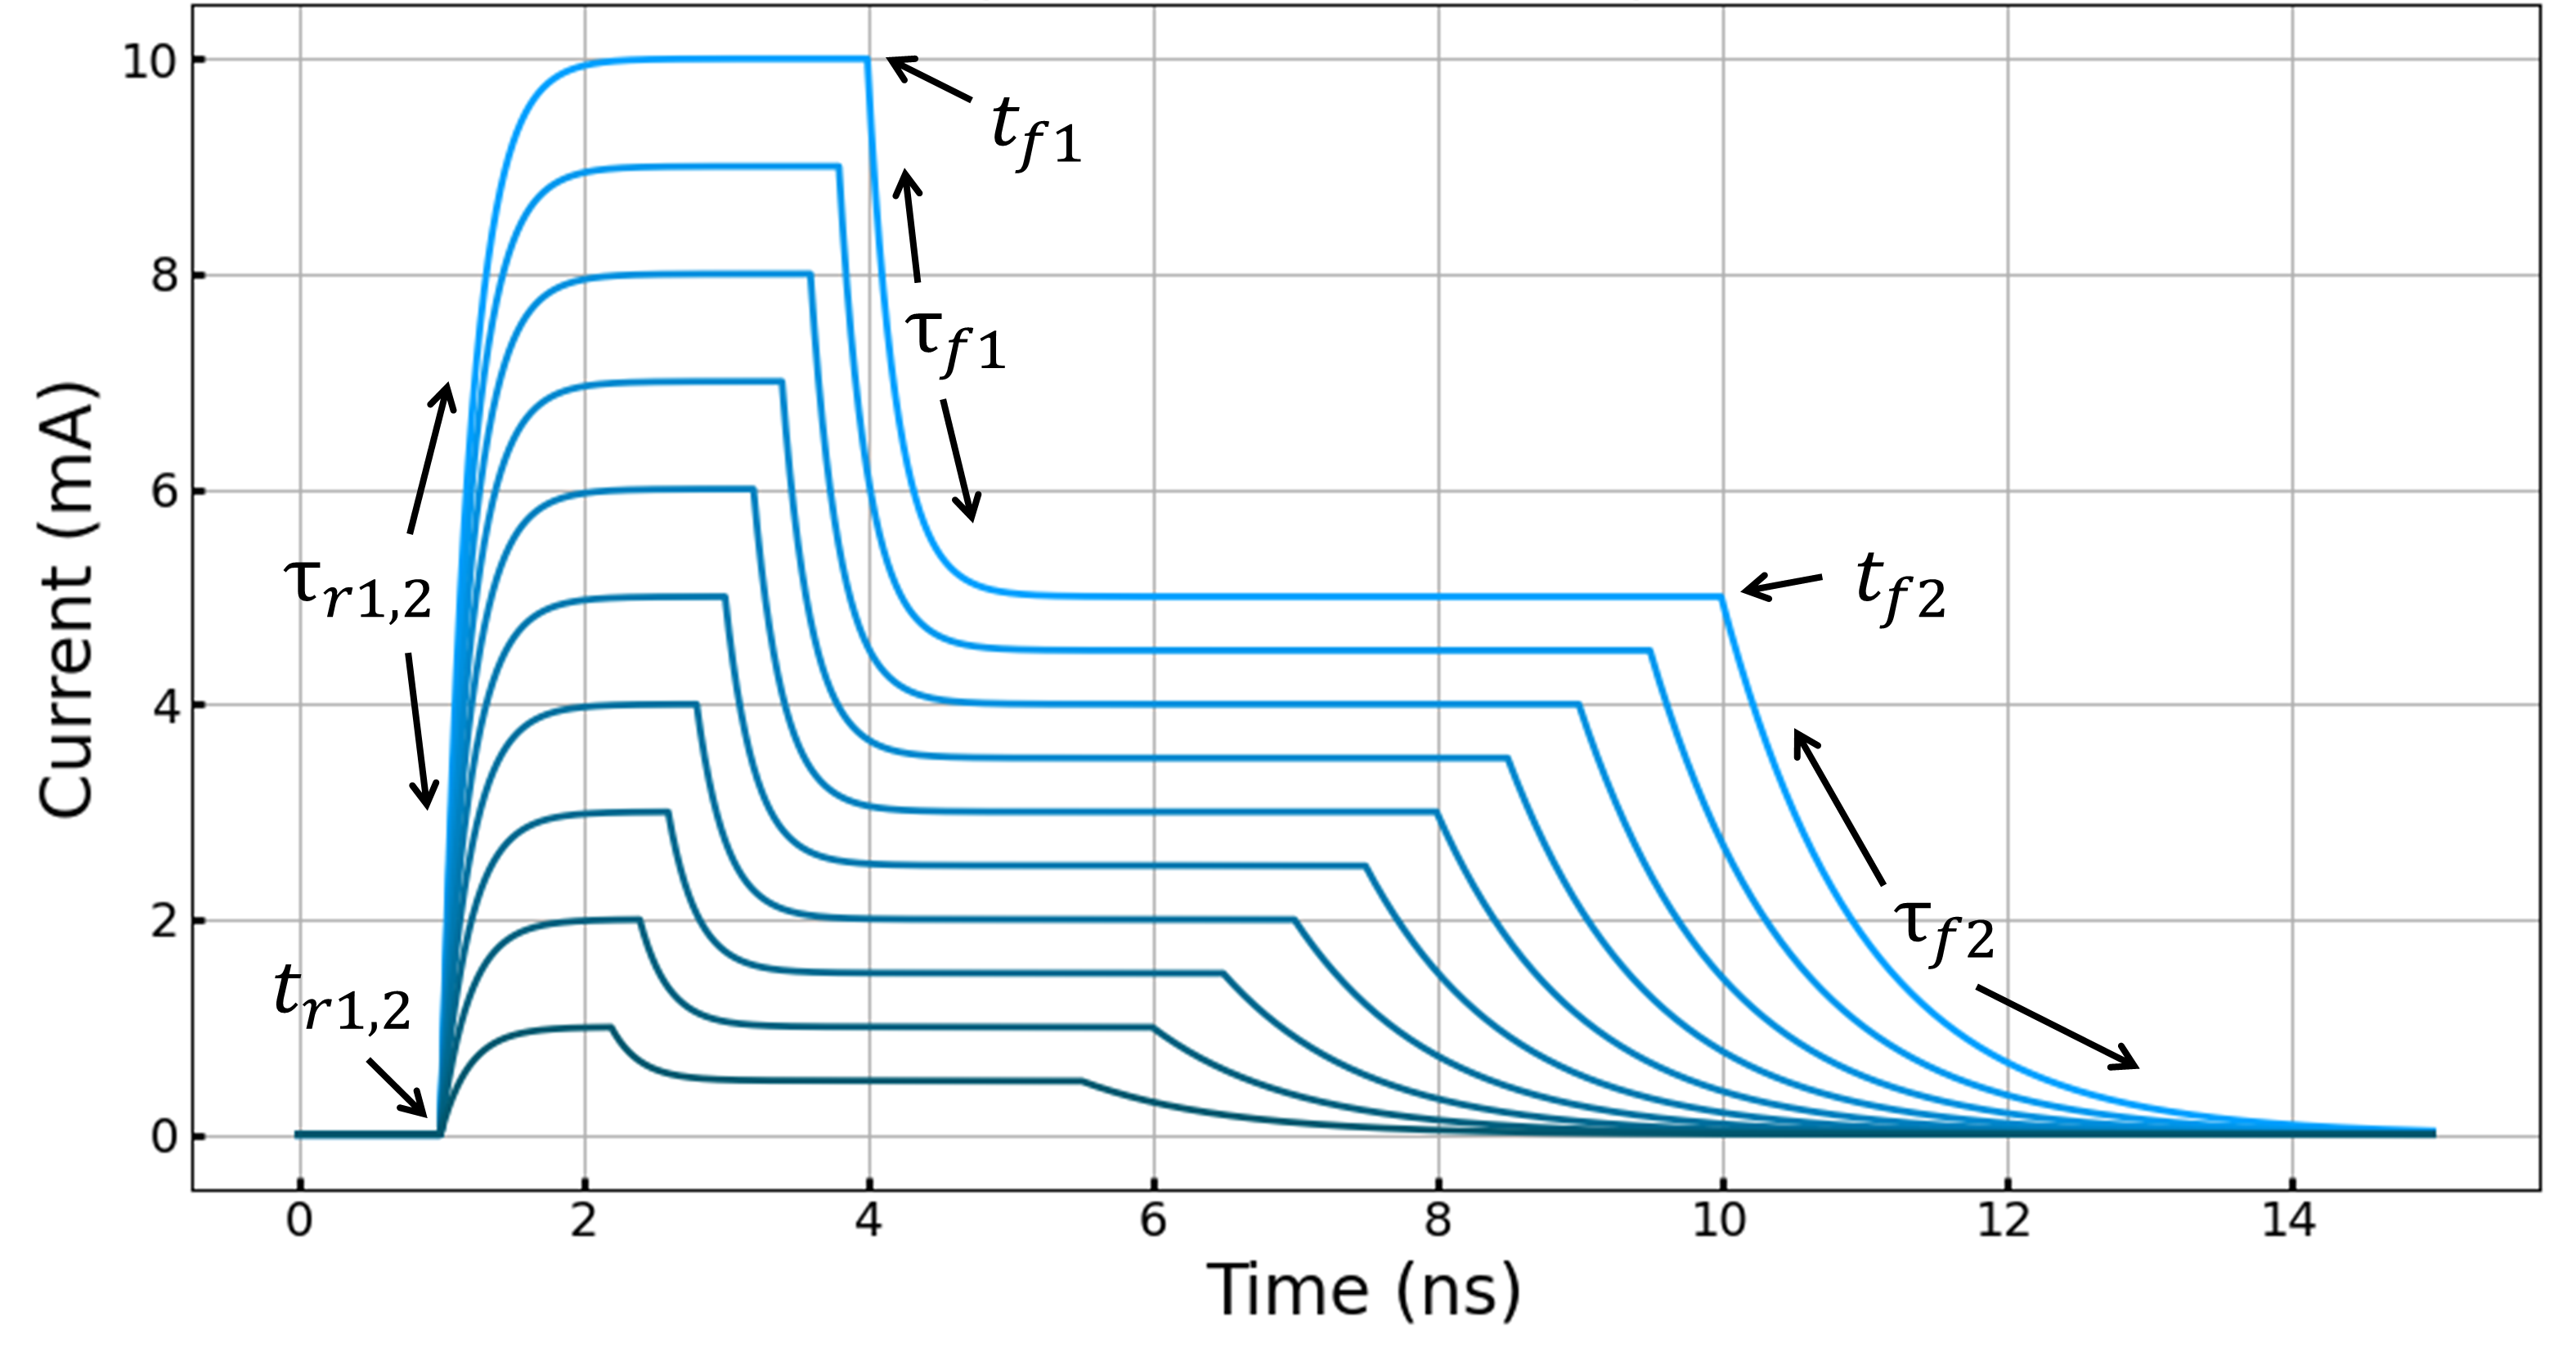
\includegraphics[width=0.95\linewidth]{dual_double_exp_param_no_title}
        \caption{Family of dual double exponential curves. The dual double exponential radiation simulation block can generate custom curves by adjusting various parameters such as \(t_{r1}\), \(t_{r2}\), \(t_{f1}\), \(t_{f2}\), \(\tau_{r1}\), \(\tau_{r2}\), \(\tau_{f1}\), and \(\tau_{f2}\).}
        \label{fig:dual_double_exp}
    \end{figure}

    \subsubsection{Adaptive Double Exponential Current Source}
    A problem that arises when using either the double or dual double exponential current models is that these models can produce unrealistic node voltages.
    If, for example, a double or dual double exponential current source is placed from the drain to the body node of a reverse biased NMOS transistor, when the current source is activated, the drain node voltage can be pulled below the ground node voltage.
    This means that the NMOS transistor is no longer held in reverse bias and no current should be flowing.

    The adaptive double exponential current source solves this problem by adjusting the drive current proportional to the voltage across the reverse bias PN junction of the transistor for which a radiation strike is being simulated for~\cite{Kauppila2009}.
    This adjustment allows the node voltage to drop to near zero and remain at this level until the radiation induced current spike is complete.
    The resulting current waveform closely resembles that of a dual double exponential current source. Fig. ~\ref{fig:adaptive_model_overview} shows how the adaptive double exponential current source is constructed.

    \begin{figure}[htbp]
        \centering
        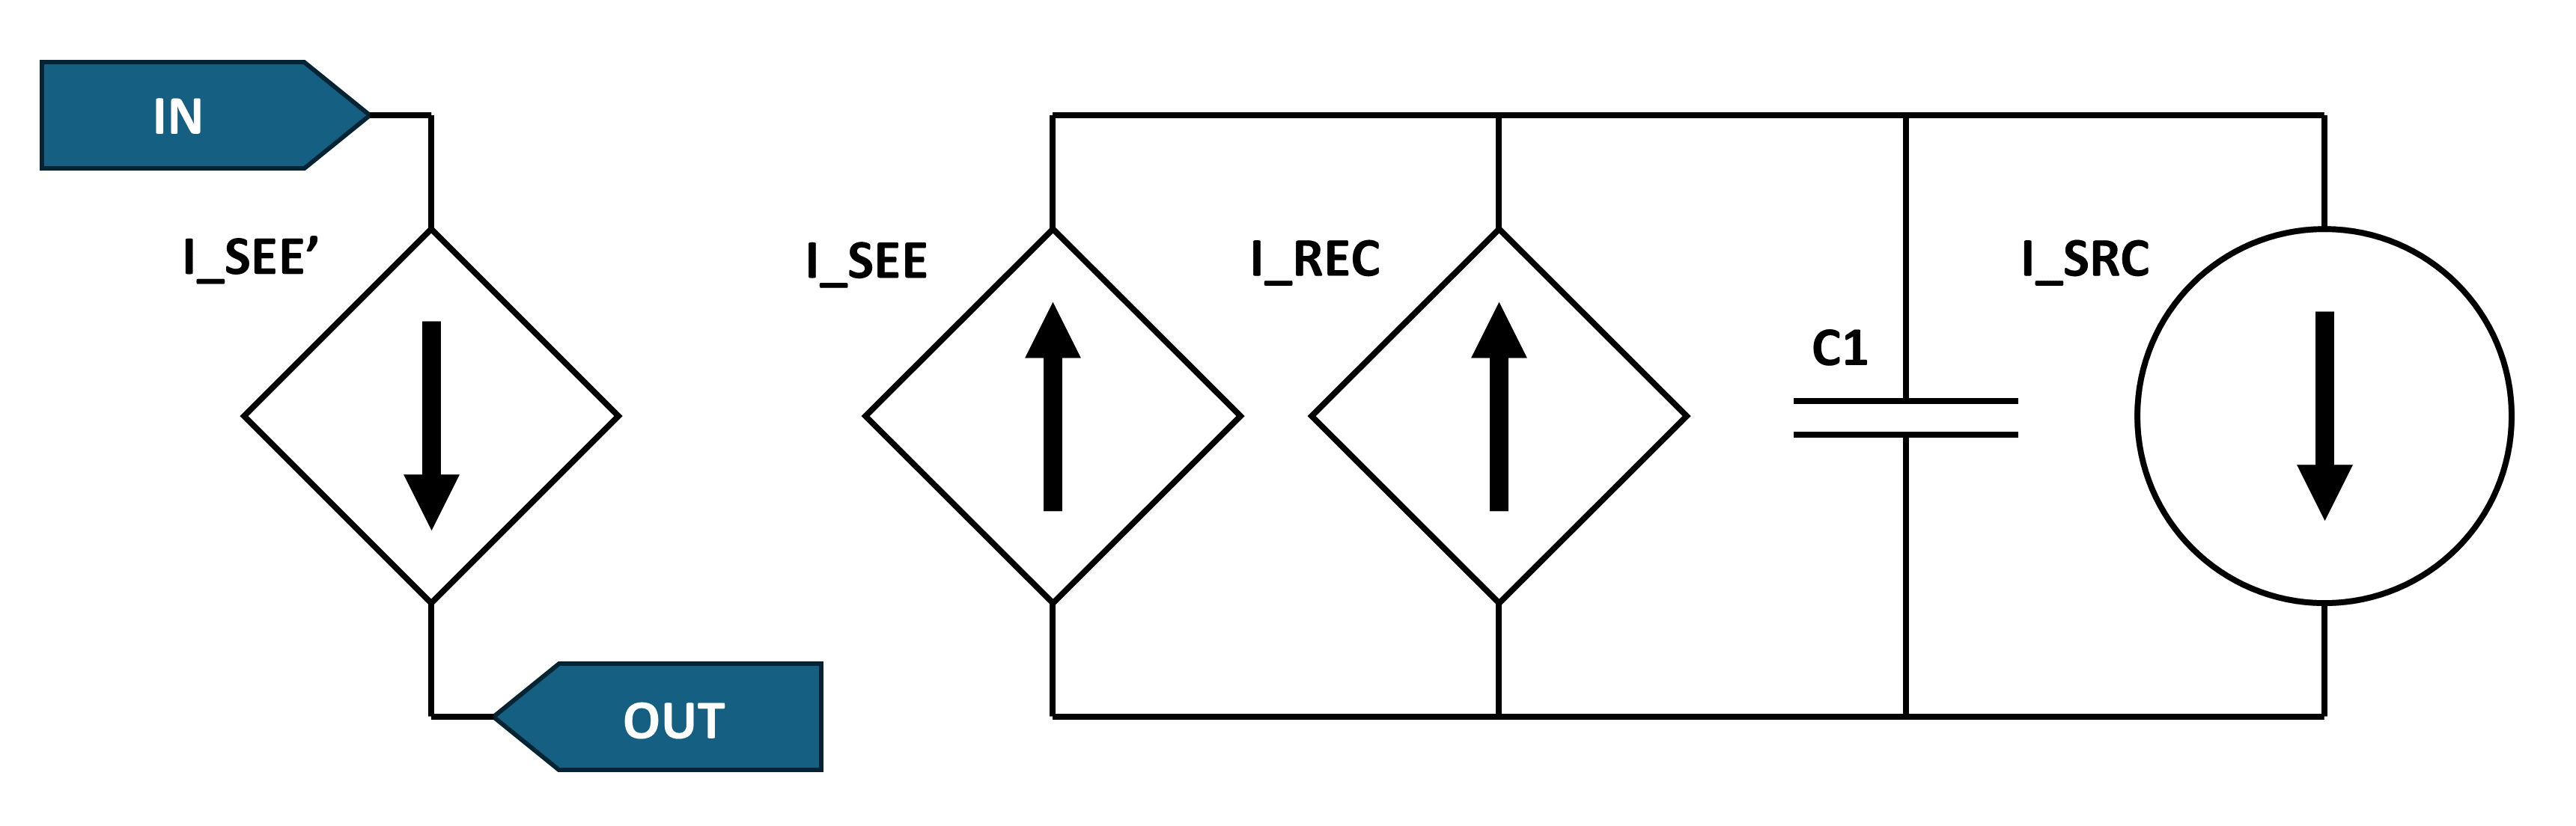
\includegraphics[width=0.95\linewidth]{Adaptive_Model_Cropped}
        \caption{Overview of adaptive double exponential current source model \cite{Kauppila2009}}
        \label{fig:adaptive_model_overview}
    \end{figure}

    The following equations define the behavior of the adaptive model:

    \begin{equation}
        I_{SEE} = Q(C1) \cdot (V(IN) - V(OUT)) \cdot k\label{eq:ISEE}
    \end{equation}

    \(I_{SEE}\) (The observed current due to single event effects) is a function of the total charge stored in the capacitor, the voltage across the adaptive current source, and an adjustment constant \(k\).

    \begin{equation}
        I_{REC} = recomb\_adj \cdot Q(C1) \cdot k\label{eq:IREC}
    \end{equation}

    \(I_{REC}\) (The current due to electron-hole pair recombination effects) is a function of an adjustment parameter \(recomb\_adj\), the total charge on the capacitor, and a second adjustment constant \(k\).
    Note, this \(k\) is the same \(k\) as presented in Equation~\ref{eq:ISEE}.

    \begin{equation}
        I_{SEE}' = I(I_{SEE})\label{eq:ISEE'}
    \end{equation}

    \(I_{SEE}'\) is a current mirror of \(I_{SEE}\).
    This allows for the calculation portion of the circuit to be separated from outside influence~\cite{Kauppila2009}.

    Lastly, \(I_{SRC}\) is the standard double exponential current source given by equations (\ref{eq:Ipeak}) and (\ref{eq:ISRC}).

    A description the additional parameters in the adaptive current source is as follows:

    \begin{itemize}
        \item[] \(k\) - A constant for proportionally adjusting the drive strength of \(I_{SEE}\) and \(I_{REC}\)

        \item[] \(recomb\_adj\) - A constant for proportionally adjusting the drive strength of \(I_{REC}\)

    \end{itemize}
    \vspace{1em}

    \subsubsection{Usage}
    To simulate a single event effect on a PMOS transistor, a single event effect simulation block must be placed with the input of the block connected to the body node of the PMOS transistor and the output of the block connected to the drain node of the PMOS transistor.

    To simulate a single event effect on an NMOS transistor, a single event effect simulation block must be placed with the input of the block connected to the drain node of the NMOS transistor and the output of the block connected to the body node of the NMOS transistor.
    
    The reason behind these configuration restraints is beyond the scope of this paper.

	\section{Example Usage}\label{sec:example-usage}
	\begin{figure}[htbp]
        \centering
        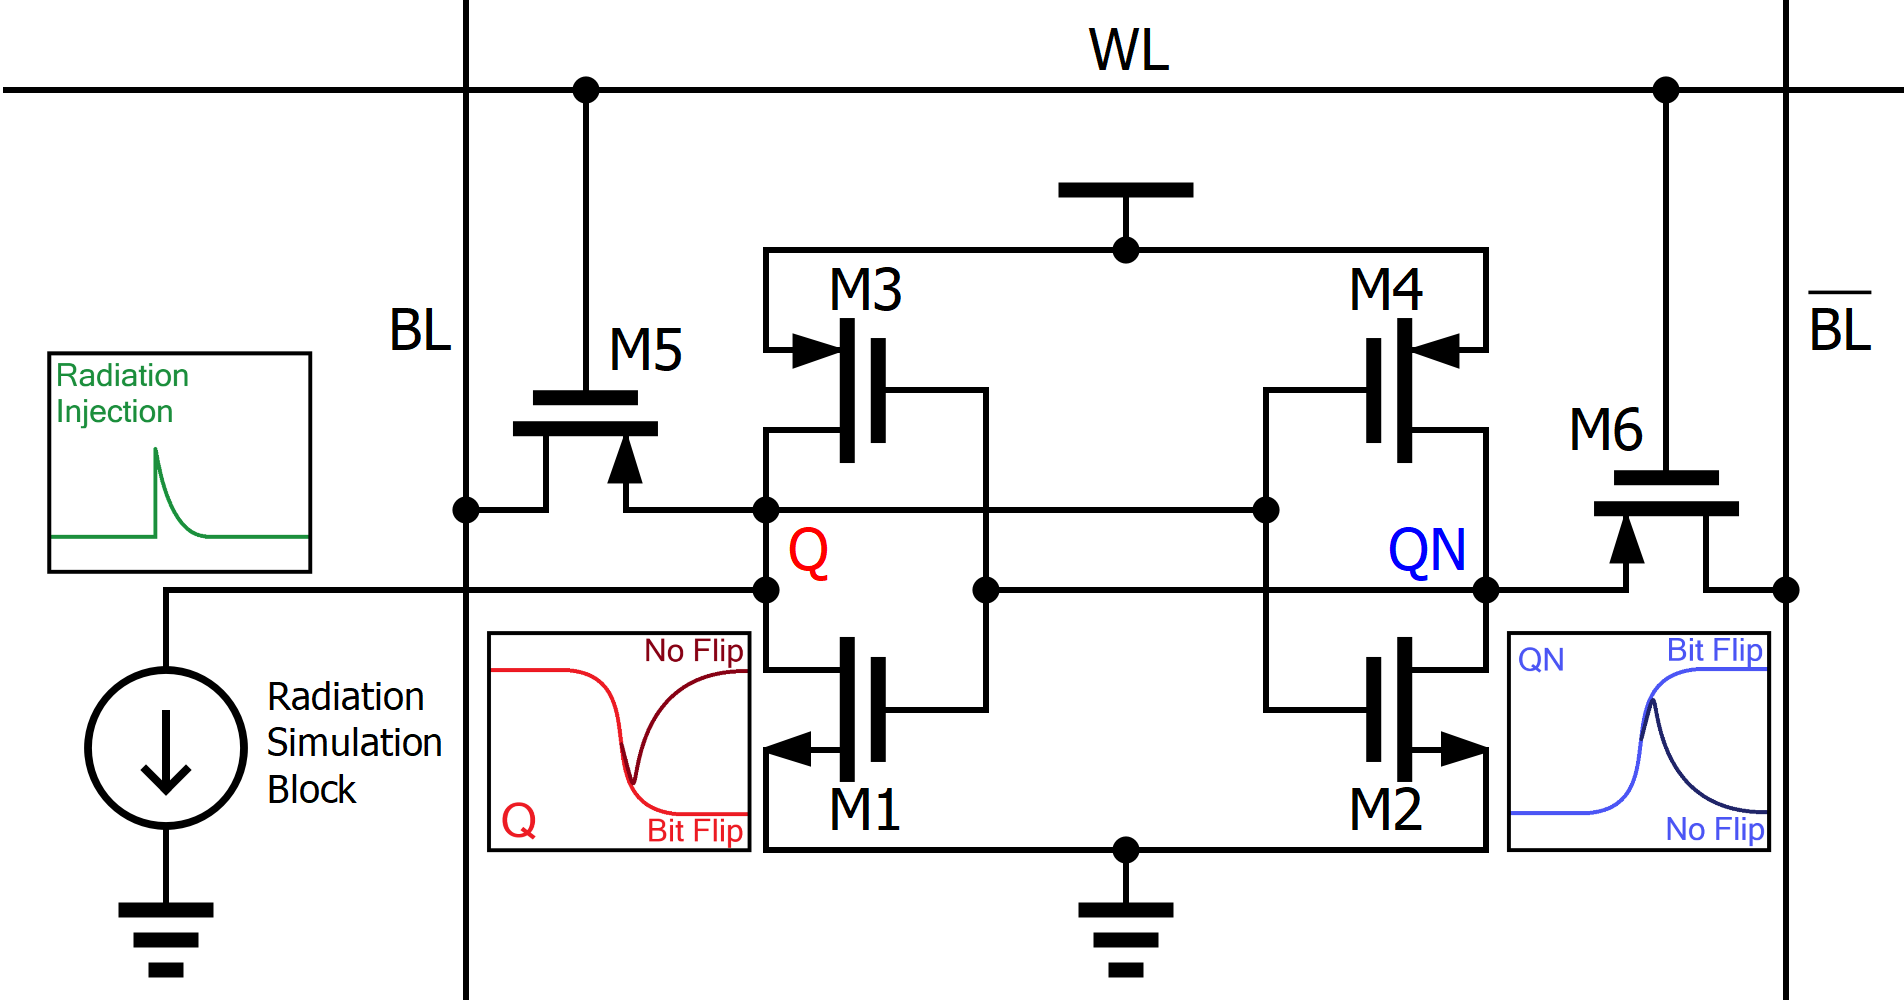
\includegraphics[width=0.95\linewidth]{small_sram}
        \caption{Example SRAM simulation. In this diagram, a radiation event occuring in the drain region of the M1 transistor is simulated by placing a radiation simulation block from the node Q to the body node of M1(ground).}
        \label{fig:motivating_example}
    \end{figure}    
    
    \subsection{SRAM Simulation}\label{subsec:sram_sim}
    In this section we will demonstrate how our simulator can be used to simulate radiation effects on a standard SRAM cell. SRAMs are susceptible to radiation induced upsets where the state of the cell can be flipped from zero to one or vice versa. To simulate a radiation strike, a schematic can be set up as seen in Fig. \ref{fig:motivating_example}. In this schematic, a radiation simulation block is placed to simulate a particle striking the drain region of the NMOS transistor on the Q side of the SRAM. The parameters of the simulation block are set according to process parameters, as well as experimental data. When the simulation is run, the radiation simulation block will inject current at a presribed time. The results of such a simulation are presented in Fig.\ref{fig:motivating_example_result}
    
    
    
    \begin{figure}[htbp]
        \centering
        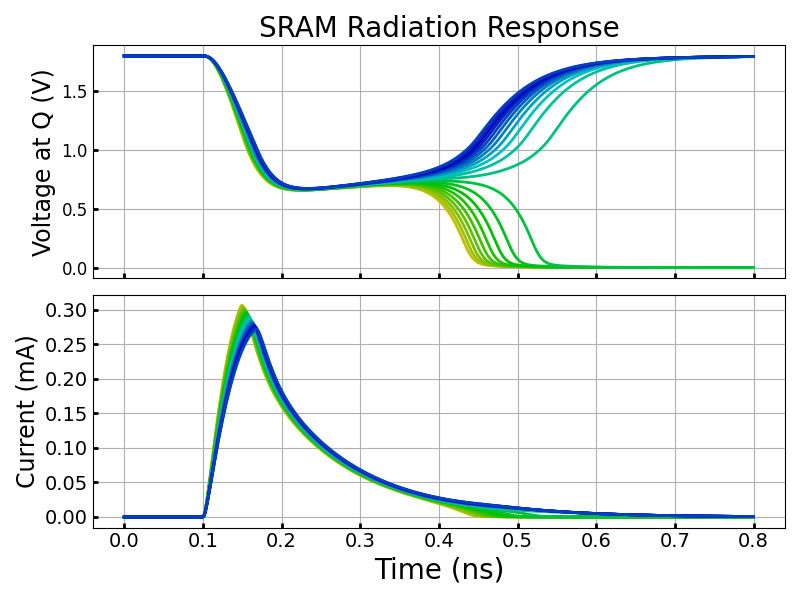
\includegraphics[width=0.95\linewidth]{SRAM_Response_Multi}
        \caption{Sram Simulation. In the above image, the voltage response of an SRAM cell to a suite of radiation simulation charge injections is shown. By adjusting the parameters of the simulation, the SRAM state was either maintained or upset.}
        \label{fig:motivating_example_result}
    \end{figure}

	From this simulation, we were able to determine the parameters for which a radiation strike will cause a single event upset in the SRAM cell, and the parameters for which an upset will not occur. This is seen in the split nature of V(Q) in Fig.~\ref{fig:motivating_example_result}.

    \section{Conclusion and Future Work}\label{sec:conclusion-and-future-work}
    This paper presented an open-source radiation hardening simulator designed to simulate and analyze the effects of radiation on electronic circuits.
    The simulator integrates XSchem and NGSpice with custom-developed modules for radiation effect simulation.
    The incorporation of advanced models for Single Event Effects has shown accuracy in preliminary tests, demonstrating the system's potential for reliable simulations.

    In future work, we plan to further optimize the simulator and explore additional features.
    We aim to enhance the simulator's capability to handle more complex scenarios and to improve its user interface for better usability.
    Additionally, we will investigate potential collaborations with other research projects to expand the simulator's applications and impact~\cite{Pepper1990}.
    Future developments will focus on refining the adaptive models and integrating more comprehensive radiation effect simulations to support a wider range of research and practical applications.

    \section*{Acknowledgment}
    The authors would like to thank Dr. Shiuh-hua Wood Chiang, Dr. Mike Wirthlin, and Dr. Jeffrey Goeders, for their guidance and support throughout this project.
    We also acknowledge the contributions of our colleagues and the funding support from the SCALE program~\cite{SCALE}.
    Their assistance has been invaluable in the development and success of this project.

    \bibliographystyle{IEEEtran}
    \bibliography{references}

\end{document}
